\section{Fundamentals}

\begin{tabular}{|l|c|c|}
\hline \textbf{Description} & \textbf{Symbol} & \textbf{Unit} \\ 
\hline Free electric charge in the system & $Q$ & $C = As$ \\
\hline Volumetric free charge density & $\rho$ & $\frac{C}{m^3}$ \\
\hline Individual electric current flowing through the surface $S$ & $I_i$ & $A$ \\
\hline Magnetic flux through the surface $S$ & $\Phi$	& $Wb = Tm^2$\\
\hline Induced voltage along the closed loop $\delta S$ & $u_i$ & $V$ \\
\hline Electric current density & $\vec{J} = \sigma \vec{E}$ & $\frac{A}{m^2}$\\
\hline Electric flux density & $\vec{D} = \varepsilon \vec{E}$ & $\frac{C}{m^2} = \frac{As}{m^2}$\\
\hline Electric field & $\vec{E} = \frac{\vec{D}}{\varepsilon}$ & $\frac{V}{m}$\\
\hline Magnetic flux density & $\vec{B} = \mu \vec{H}$ & $T = \frac{Vs}{m^2}$\\
\hline Magnetic field & $\vec{H} = \frac{\vec{B}}{\mu}$ & $\frac{A}{m}$\\
\hline Electric permittivity & $\varepsilon = \varepsilon_0 \varepsilon_r$ & $\varepsilon_0 = 8.85 \cdot 10^{-12} \left[\frac{F}{m} = \frac{As}{Vm}\right]$\\
\hline Magnetic permeability & $\mu = \mu_0 \mu_r$ & $\mu_0 = 4\pi \cdot 10^{-7} \left[\frac{Tm}{A} = \frac{H}{m} = \frac{Vs}{Am}\right]$ \\
\hline 
\end{tabular} 

\textbf{\\ \\ Gradient\\ \\}
\begin{minipage}[lt]{5cm}
	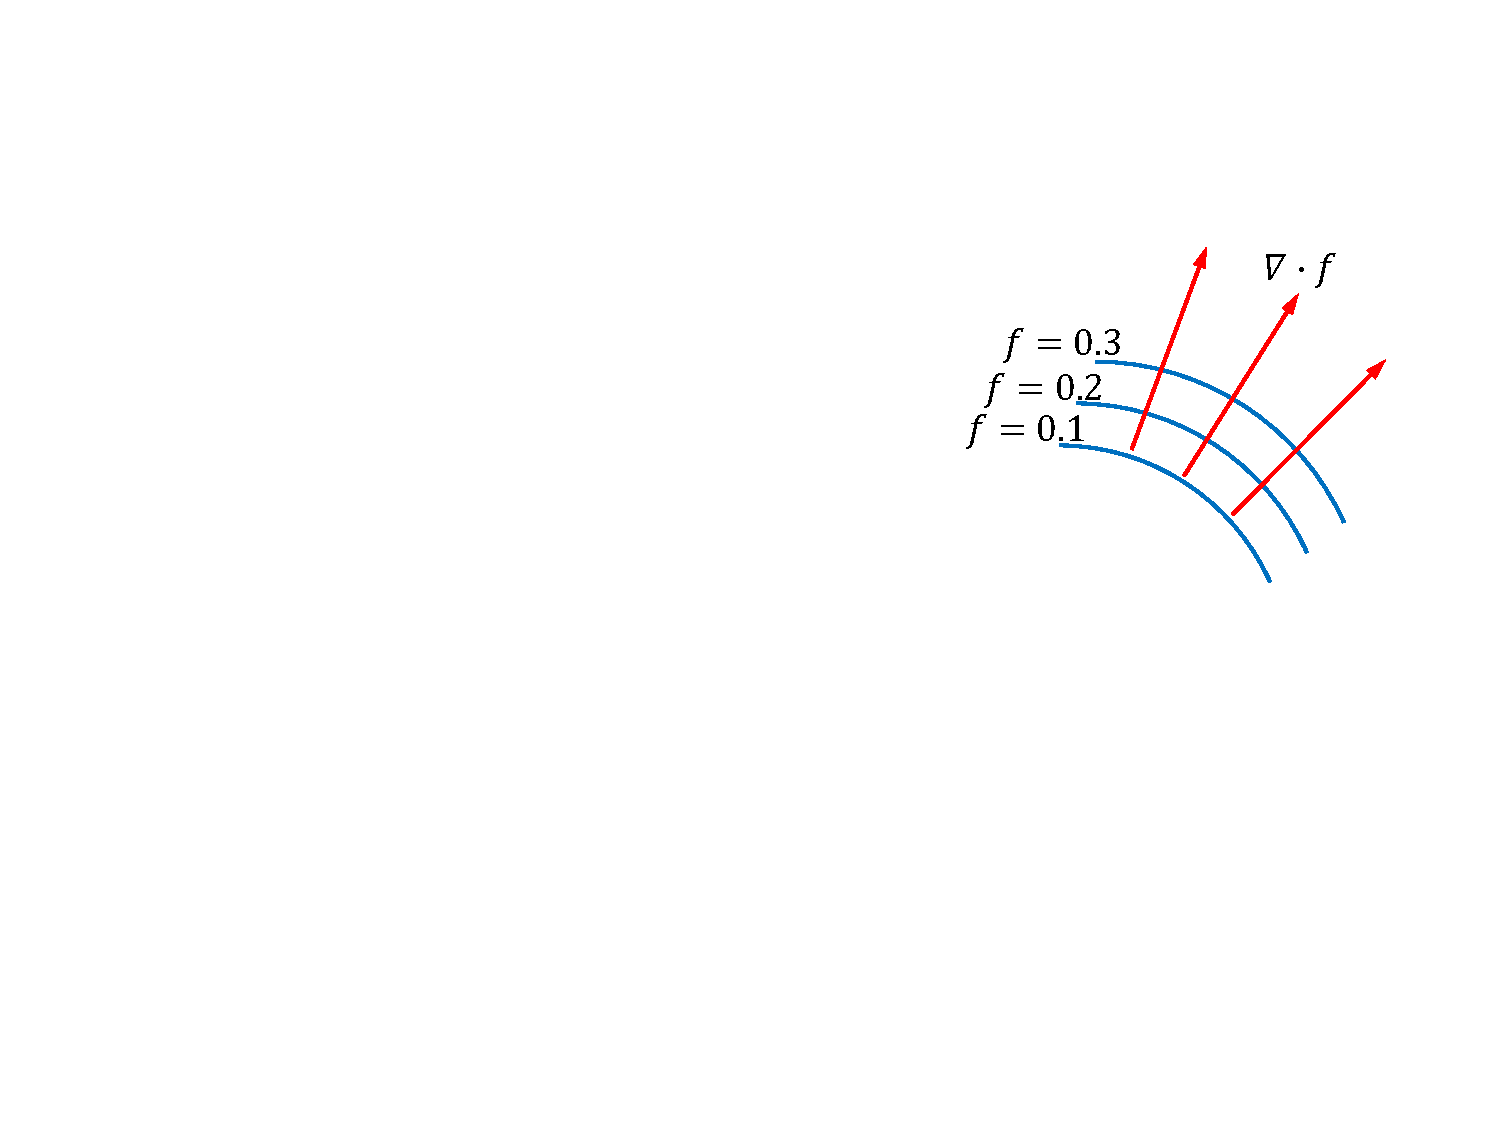
\includegraphics[width=.8\textwidth]{./images/Gradient.pdf}
\end{minipage}
\begin{minipage}[rt]{13cm}
	The gradient of a scalar field reveals the direction of the steepest ascent of the scalar function (perpendicular to the corresponding isolines of the function). \\ \\
	\begin{tabular}{ll}
		Scalar field: & \(\displaystyle f = f\left(\vec{r}\right) = f\left(x,y,z\right) \) \\ 
		Gradient is a vector: & \(\displaystyle \textrm{grad }f = \lim\limits_{\textrm{diameter}\left(D\right)\rightarrow 0} \frac{\oiint_{\textrm{boundary}\left(D\right)}f \cdot \vec{dA}}{\textrm{measure}\left(D\right)}, D\subseteq R^3 \) \\
		Gradient in Cartesian coordinates: & \(\displaystyle \textrm{grad }f = \frac{\partial f}{\partial x} \cdot \vec{e_x}+\frac{\partial f}{\partial y} \cdot \vec{e_y}+\frac{\partial f}{\partial z} \cdot \vec{e_z} \) \\ 
		$\nabla$-operator (Nabla): & \(\displaystyle \nabla = \frac{\partial}{\partial x} \cdot \vec{e_x}+\frac{\partial}{\partial y} \cdot \vec{e_y}+\frac{\partial}{\partial z} \cdot \vec{e_z} \)\\
		Gradient and $\nabla$-operator: & \(\displaystyle \textrm{grad }f = \nabla \cdot f \)\\
	\end{tabular} 
\end{minipage}

\textbf{\\ \\ Divergence\\ \\}
\begin{minipage}[lt]{5cm}
	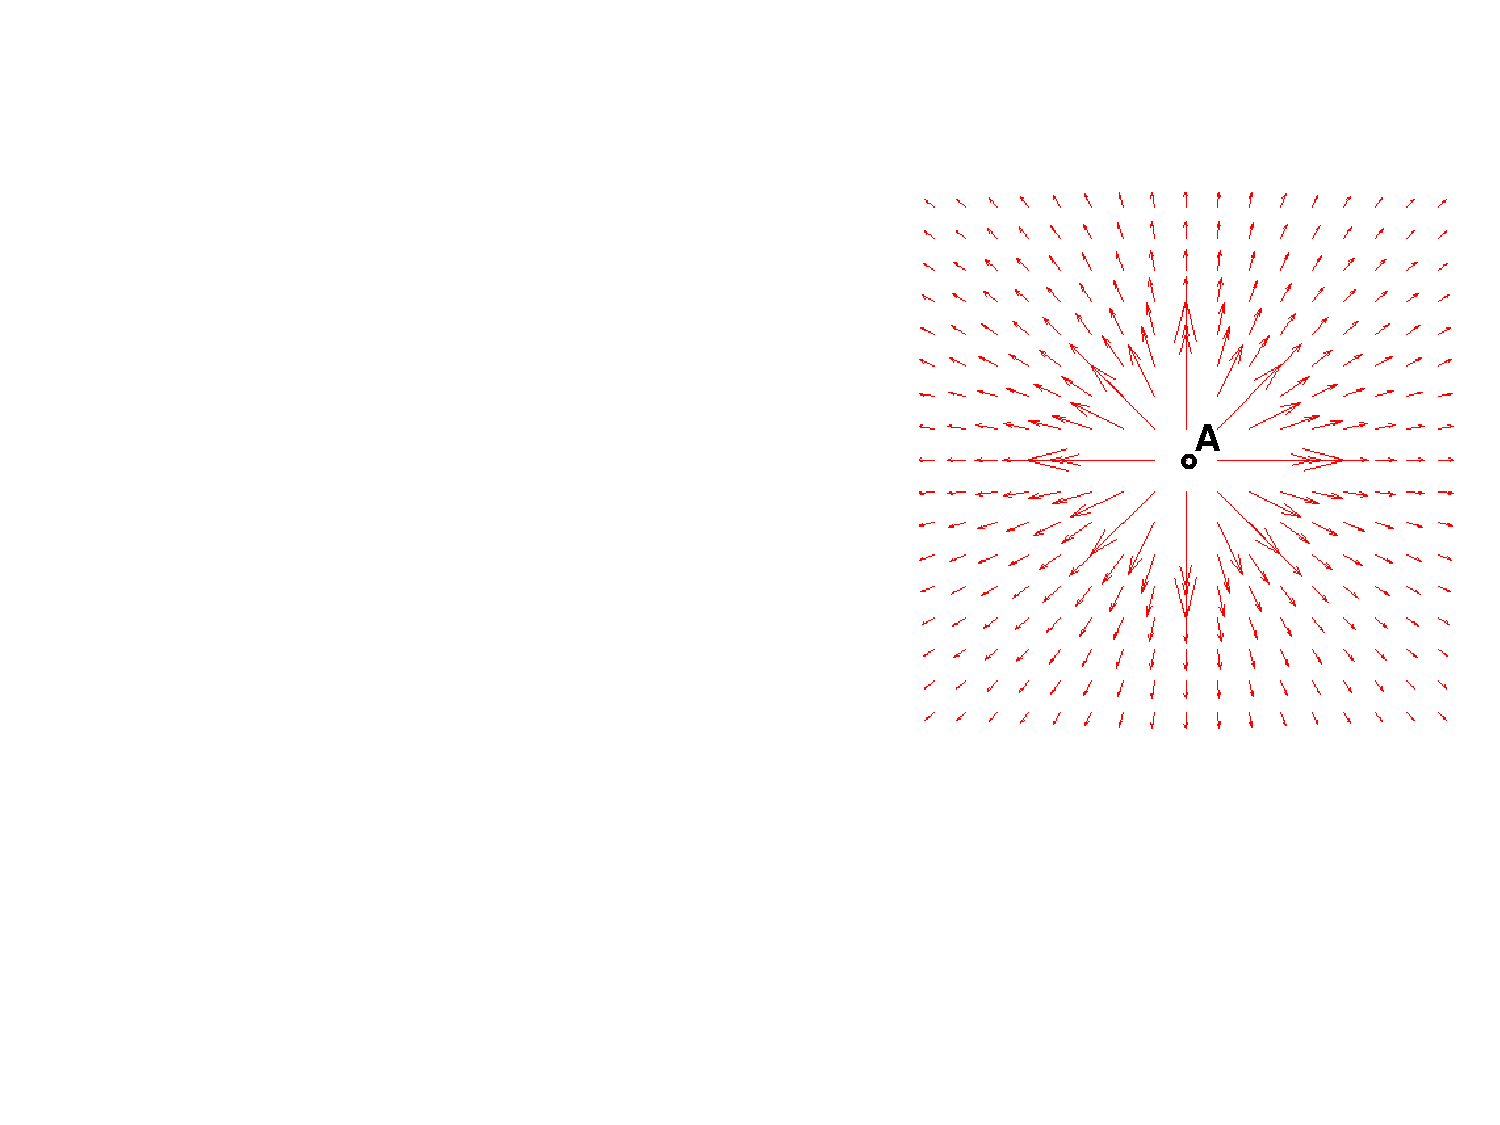
\includegraphics[width=.8\textwidth]{./images/Divergence.pdf}
\end{minipage}
\begin{minipage}[rt]{13cm}
	In the central point $A$ of this field distribution is: $div \vec{a} > 0$. Generally speaking, a positive or negative divergence reveals a field source or a field sink, respectively. \\ \\
	\begin{tabular}{ll}
		Vector field: & \(\displaystyle \vec{a} = \vec{a}\left(\vec{r}\right) = \vec{a}\left(x,y,z\right)\) \\
		Divergence is a scalar: & \(\displaystyle div~\vec{a} = \lim\limits_{\textrm{diameter}\left(D\right)\rightarrow 0} \frac{\oiint_{\textrm{boundary}\left(D\right)} \vec{a} \cdot \vec{dA}}{\textrm{measure}\left(D\right)}, D\subseteq R^3\) \\
		Divergence in Cartesian coordinates: & \(\displaystyle div~\vec{a} = \frac{\partial a_x}{\partial x} + \frac{\partial a_y}{\partial y} + \frac{\partial a_z}{\partial z} \)\\
		Divergence and $\nabla$-operator: & \(\displaystyle div~\vec{a} = \nabla \cdot \vec{a} \) \\
	\end{tabular}
\end{minipage}

\textbf{\\ \\ Curl\\ \\}
\begin{minipage}[lt]{5cm}
	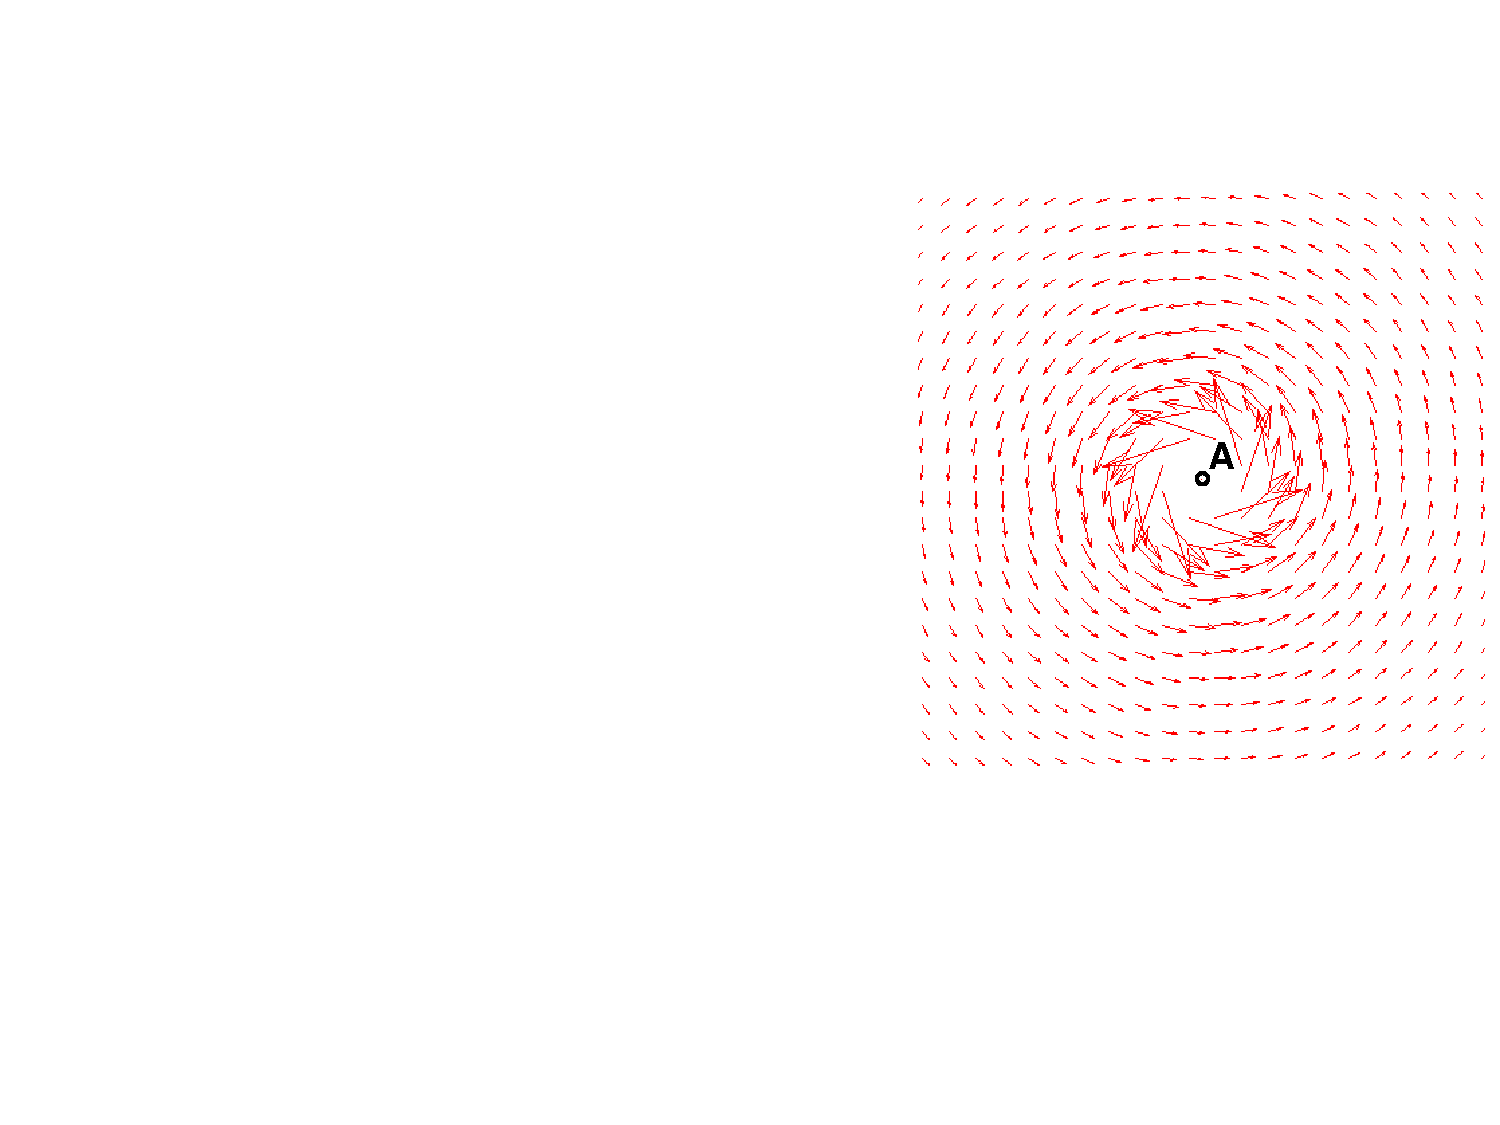
\includegraphics[width=.8\textwidth]{./images/Curl.pdf}
\end{minipage}
\begin{minipage}[rt]{13cm}
	In the central point $A$ of this field distribution is: $curl \vec{a} > 0$. Generally speaking non-zero curl reveals a rotational field character. (Curl looks what stays in this area).\\ \\
	\begin{tabular}{ll}
		Vector field: & \(\displaystyle \vec{a} = \vec{a}\left(\vec{r}\right) = \vec{a}\left(x,y,z\right)\)\\
		Curl is a vector: & \(\displaystyle \textrm{curl }\vec{a} = \lim\limits_{\textrm{diameter}\left(D\right)\rightarrow 0} \frac{\oiint_{\textrm{boundary}\left(D\right)} \vec{dA} \times \vec{a}}{\textrm{measure}\left(D\right)}, D\subseteq R^3\)\\
		Curl in Cartesian coordinates: & \(\displaystyle \textrm{curl }\vec{a} = 
		\begin{vmatrix}
			\vec{e_x} & \vec{e_y} & \vec{e_z} \\
			\frac{\partial}{\partial x} & \frac{\partial}{\partial y} & \frac{\partial}{\partial z} \\
			a_x & a_y & a_z \\
		\end{vmatrix}\) {\tiny \texttt{other coordinates in Bronstein: P.719ff}}\\
		& \(\displaystyle = \vec{e_x}\frac{\partial}{\partial y}a_z +   		\vec{e_y}\frac{\partial}{\partial z}a_x +\vec{e_z}\frac{\partial}{\partial x}a_y - \vec{e_x}\frac{\partial}{\partial z}a_y - \vec{e_y}\frac{\partial}{\partial x}a_z - \vec{e_z}\frac{\partial}{\partial y}a_x\) \\
		Curl and $\nabla$-operator: & \(\displaystyle \textrm{curl }\vec{a} = \nabla \times \vec{a} \) \\
	\end{tabular}
\end{minipage}

\textbf{\\ \\ Irrotationality of electrostatic field \\}
\begin{minipage}[lt]{9cm}
	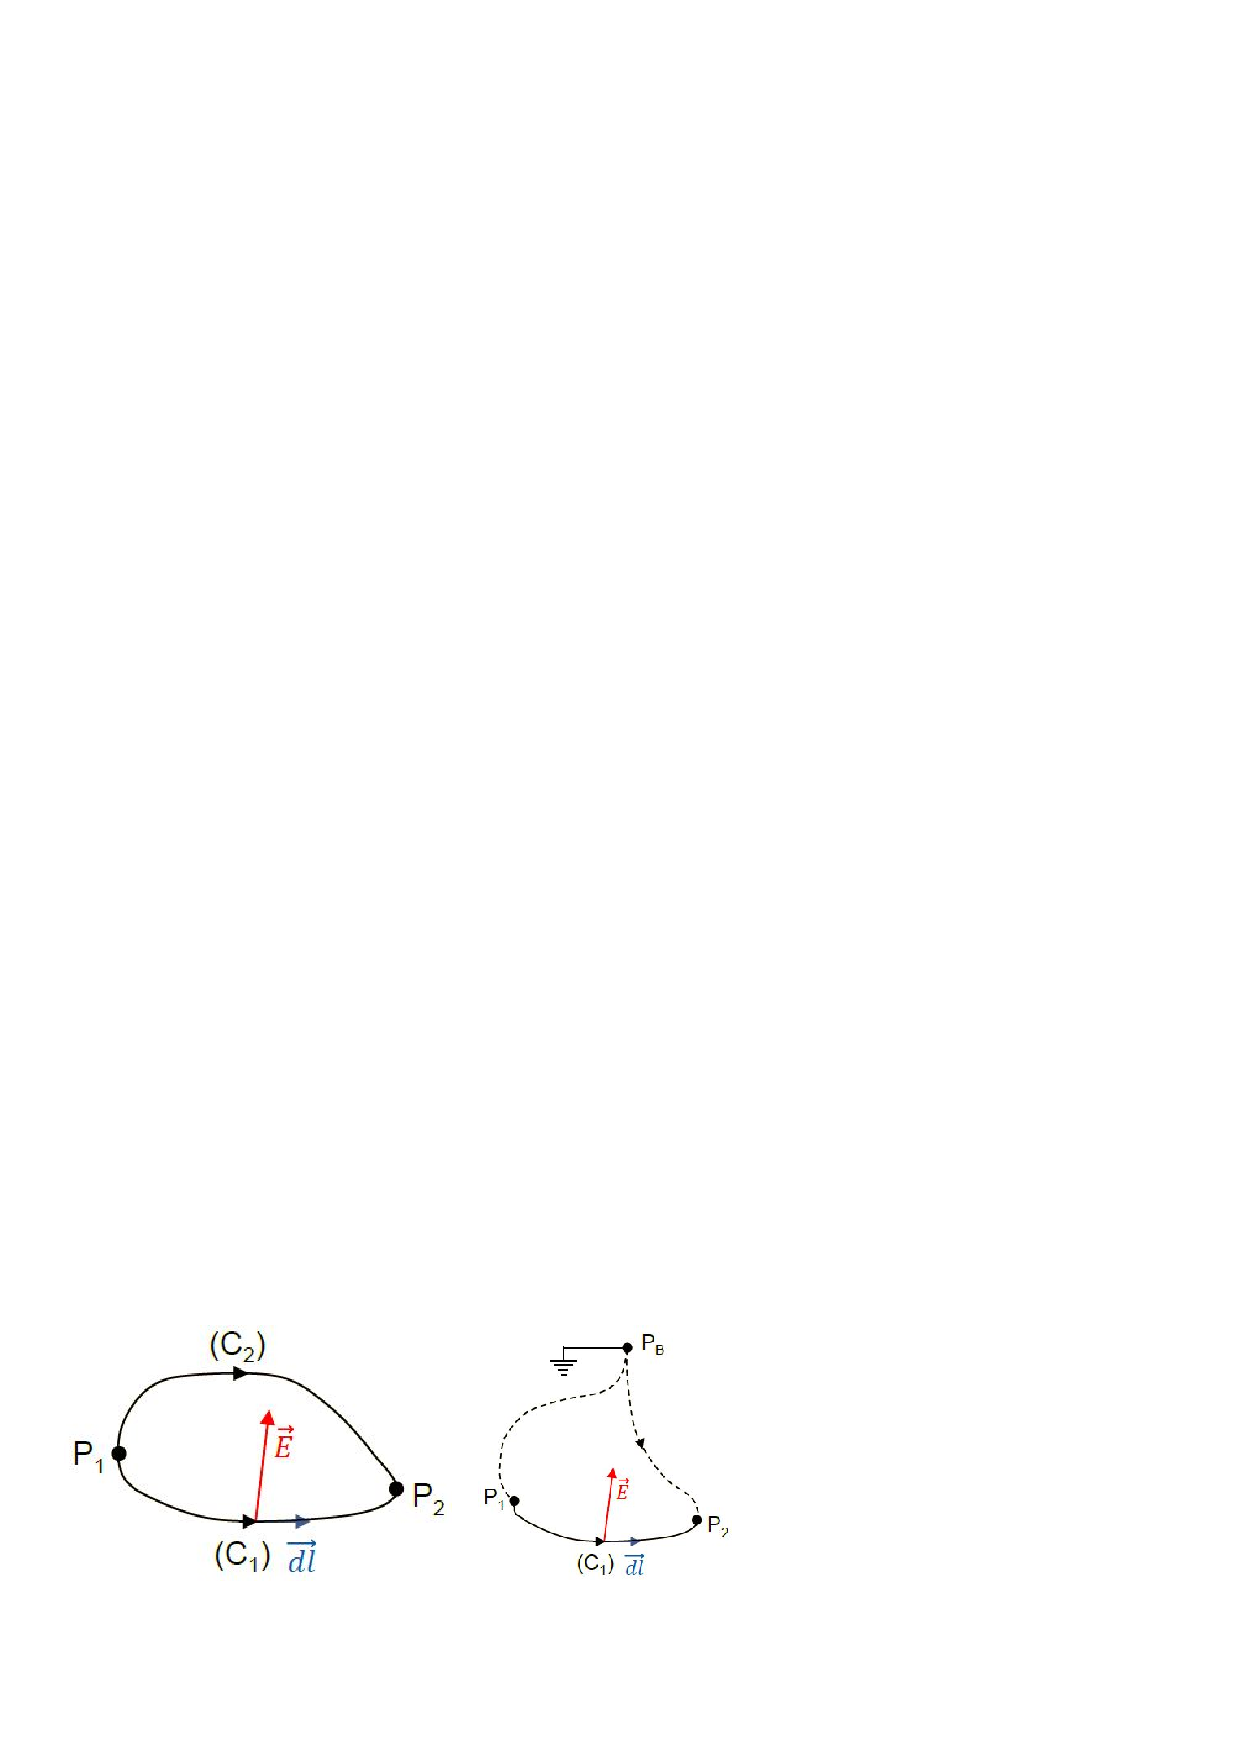
\includegraphics[width=.9\textwidth]{./images/WirbelfreiE2.pdf}
\end{minipage}
\begin{minipage}[rt]{10cm}
	\begin{equation*}
		\oint \limits_{\left(C\right)} \vec{E}\cdot \vec{dl} = 0
	\end{equation*}
	\begin{equation*}
		\int\limits_{\left(C\right)} \vec{E} \cdot \vec{dl} = \underbrace{\int_{P_1}^{P_2} \vec{E} \cdot \vec{dl}}_{C_1} - \underbrace{\int_{P_1}^{P_2} \vec{E} \cdot \vec{dl}}_{C_2} = 0
	\end{equation*}
	\begin{equation*}
		V_{P_1P_2} = \varphi_{P_1} - \varphi_{P_2} = \int_{P_1}^{P_B} \vec{E} \cdot \vec{dl} - \int_{P_1}^{P_B} \vec{E} \cdot \vec{dl} = \int_{P_1}^{P_2} \vec{E} \cdot \vec{dl}
	\end{equation*}
\end{minipage}
The line integral of an electrostatic field only depends on the start and end point. It is independent of the chosen path (conservative field).

\textbf{\\ \\ Theorems\\}
	Gauss theorem:
	\begin{equation*}
		\oiint\limits_{\left(\partial \Omega\right)} \vec{a} \cdot d\vec{S} = \iiint\limits_{\left(\Omega\right)} \nabla \cdot \vec{a} \cdot dV
	\end{equation*}
	Stokes theorem:
	\begin{equation*}
		\int\limits_{\left(\partial S\right)} \vec{a} \cdot d\vec{l} = \iint\limits_{\left(S\right)} \nabla \times \vec{a} \cdot d\vec{S}
	\end{equation*}
	
\textbf{\\ \\Continuity Equation\\}
	The current through a closed oriented surface $(S)$ can be computed as
	\begin{equation*}
		I = \oiint\limits_{\left(S\right)} \vec{J} \cdot \vec{dS}
	\end{equation*}
	Because of conservation the outflowing current must be equal to the decreasing total charge in volume $(V)$.
	\begin{equation*}
		I = -\frac{dQ}{dt} = -\frac{d}{dt}\iiint\limits_{\left(V\right)} \rho \cdot dV = -\iiint\limits_{\left(V\right)} \frac{d \rho}{dt}dV
	\end{equation*}
	Both combined leads to the Continuity Equation
	\begin{equation*}
		\oiint\limits_{\left(S\right)} \vec{J} \cdot \vec{dS} = - \iiint\limits_{\left(V\right)} \frac{d\rho}{dt}dV \rightarrow \nabla \cdot \vec{J} = -\frac{\partial \rho}{\partial t}
	\end{equation*}

\textbf{\\ Ohmic law\\}
\begin{minipage}[lt]{11cm}
	\begin{tabular}{l}
		\(\displaystyle dI = \frac{dU}{R} = G \cdot dU = \sigma \cdot \frac{dA}{l} \cdot dU \) \\
		\(\displaystyle G = \sigma \cdot \frac{dA}{l} \hspace{2cm} R = \rho \cdot \frac{l}{s} \) \\
		\(\displaystyle J \cdot dA = \sigma \cdot \frac{dA}{l} \cdot E \cdot l \rightarrow J = \sigma \cdot E \) \\
		or as vectors: \(\displaystyle \vec{J} = \sigma \cdot \vec{E}\)
	\end{tabular}
\end{minipage}
\begin{minipage}[rt]{8cm}
	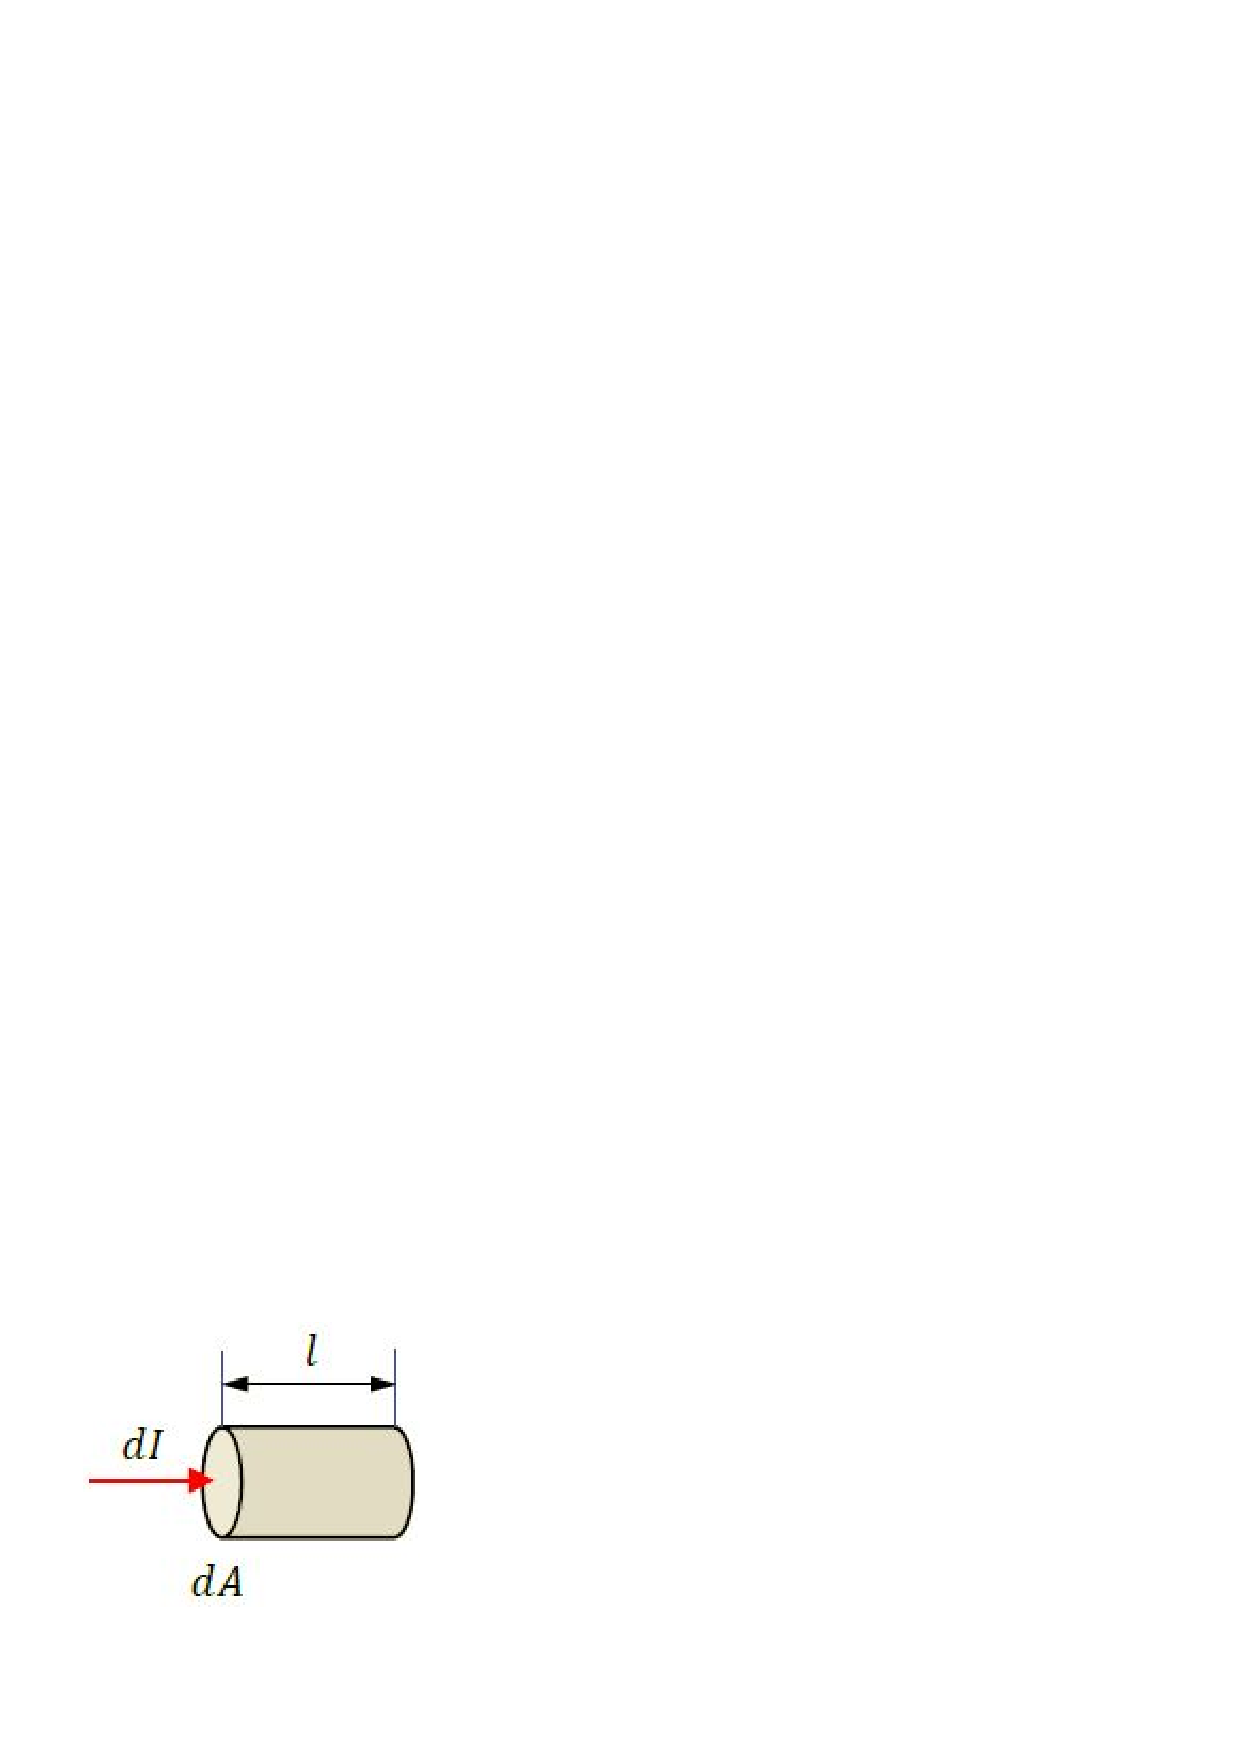
\includegraphics[width=.5\textwidth]{./images/ohmic.pdf}
\end{minipage}


\textbf{\\ \\ Rules \\}
\begin{tabular}{ll}
	Curl of a gradient is always equal to zero: & \(\displaystyle \nabla \times \left(\nabla \cdot \vec{a} \right) \equiv 0\) \\
	Divergence of a curl is always equal to zero: & \(\displaystyle \nabla \cdot \left(\nabla \times \vec{a}\right) \equiv 0 \)\\
\end{tabular}

\textbf{\\ \\ Operators \\} 
\begin{tabular}{ll}
	Laplace Operator: & \(\displaystyle \nabla \cdot \nabla = \nabla^2 = \Delta = \frac{\partial^2}{\partial x^2}+\frac{\partial^2}{\partial y^2}+\frac{\partial^2}{\partial z^2} \) \\
\end{tabular}
